%% ID: ballistic_pendulum
%% TITLE: A Ballistic Pendulum
%% TYPE: question
%% QUESTIONTYPE: numeric
%% CONCEPTS: energy, momentum, momentumii
%% VIDEOS: 
%% LEVEL: 4
%% TOPIC: mechanics/dynamics
%% ORDER: 5


\begin{problem}[HSC1929PIIQ2pa] % metric units added (numbers need checking; quite a straightforward conservation of energy / angular momentum question)
{A block of wood weighing \valuedef{M}{2.5}{kg} is suspended from fixed pegs by vertical strings \valuedef{l}{3}{m} long, in a set up known as a ballistic pendulum.  A bullet weighing \valuedef{m}{10}{g} and moving horizontally with a velocity \valuedef{u}{300}{m\,s\sup{-1} enters and remains in the block.  Find the angle through which the block swings.
}{
\stress{Adapted with permission from UCLES, Higher School Certificate Physics, June 1929, Paper 2, Question 2.}
}{
The initial situation is shown in Figure \ref{fig:Dynamics_ballistic}:
\begin{figure}[h]
	\centering
	
\includegraphics[width=9cm]{../../../figures/Dynamics_ballistic.svg}
	\caption{}\label{fig:Dynamics_ballistic}
\end{figure}
\\
After the collision the body has total mass \vari{M+m} so conserving momentum we can find an expression for the speed after impact \vari{v}:
\begin{eqnarray*}
mu&=(M+m)v \\
\Rightarrow v&=\frac{m}{M+m}u
\end{eqnarray*}
We can then conserve energy to find the required angle. Figure \ref{fig:Dynamics_ballistictwo} shows the final position with the block at rest:
\begin{figure}[h]
	\centering
	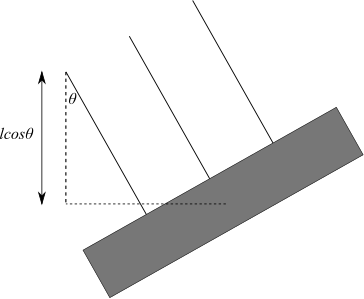
\includegraphics[width=9cm]{../../../figures/Dynamics_ballistictwo.svg}
	\caption{}\label{fig:Dynamics_ballistictwo}
\end{figure}
\\
The initial kinetic energy is all converted to gravitational potential energy so
\begin{eqnarray*}
\frac{1}{2}(M+m)v^2=(M+m)gh
\end{eqnarray*} 
The change in height of the centre of mass of the block, assuming the distance to its CoM from the point of rotation is \valuedef{l}{3}{m}, is given by \vari{h} $=$ \valuedef{l-l\cos\theta}{l(1-\cos\theta)}{}. Therefore
\begin{eqnarray*}
\frac{1}{2}(M+m)\cdot\left(\frac{mu}{M+m}\right)^2&=(M+m)gl(1-\cos\theta) \\
\Rightarrow \frac{1}{2gl}\frac{m^2u^2}{(M+m)^2}&=1-\cos\theta \\
\Rightarrow \theta&=\arccos\left(1-\frac{1}{2gl}\frac{m^2u^2}{(M+m)^2}\right)
\end{eqnarray*}
And the numerical answer is \valuedef{\theta}{12.7^\circ}{}. 
}
\end{problem}